\documentclass[a4paper,14pt]{article} % формат документа

\usepackage{cmap} % поиск в ПДФ
\usepackage[T2A]{fontenc} % кодировка
\usepackage[utf8]{inputenc} % кодировка исходного текста
\usepackage[english,russian]{babel} % локализация и переносы
\usepackage[left = 2cm, right = 1cm, top = 2cm, bottom = 2 cm]{geometry} % поля
\usepackage{listings}
\usepackage{graphicx} % для вставки рисунков
\usepackage{amsmath}
\graphicspath{{pictures/}}
\DeclareGraphicsExtensions{.pdf,.png,.jpg}
\newcommand{\anonsection}[1]{\section*{#1}\addcontentsline{toc}{section}{#1}}

\lstset{ %
	language=Python,                % Язык программирования 
	numbers=left,                   % С какой стороны нумеровать          
	frame=single,                    % Добавить рамку
}

\begin{document}
	\begin{titlepage}

       		\begin{center}
         		\large
		
        			Государственное образовательное учреждение высшего профессионального образования\\
       			“Московский государственный технический университет имени Н.Э.Баумана”
         		\vspace{3cm}
            
            		\textsc{Дисциплина: Анализ алгоритмов}
           		\vspace{0.5cm}
                
            		\textsc{Лабораторная работа № 2}
           		 \vspace{3cm}
            
           		 \LARGE 
		 
		 	Трудоемкость алгоритмов умножения матриц
           		 \vspace{3cm}
            
            		\begin{flushright}
            			Студент: \\
				Сиденко Анастасия Генадьевна \\   
            			Группа: ИУ7-53Б \\
           			\hfill
            
           			Преподаватели: \\
				Строганов Юрий Владимирович \\
           			Волкова Лилия Леонидовна
            			\vfill
            		\end{flushright}
		
			\large
            		2019 г.
		\end{center}

	\end{titlepage}
    
	\tableofcontents
	
	\newpage
    
	\anonsection{Введение}
	\hfill
	
	Матрицы упоминались ещё в древнем Китае, называясь тогда «волшебным квадратом». Основным применением матриц было решение линейных уравнений. Также волшебные квадраты были известны чуть позднее у арабских математиков, примерно тогда появился принцип сложения матриц. Сама теория матриц начала своё существование в середине XIX века. Термин «матрица» ввел Джеймс Сильвестр в 1850 г. Сегодня матрицы применяются уже не только при решении линейных уравнений. [1]
	
	Умножение матриц — это один из базовых алгоритмов, который широко применяется в различных численных методах, и в частности в алгоритмах машинного обучения. Многие реализации прямого и обратного распространения сигнала в сверточных слоях нейронной сети базируются на этой операции. [2] В физике и других прикладных науках матрицы – являются средством записи данных и их преобразования.[4] В программировании – в написании программ, массивы. Широкое применение в компьютерной графике: любая картинка на экране – это двумерная матрица, элементами которой являются цвета точек, а также матрицы используются для преобразования фигур. [5]
	
	В психологии понимание термина сходно с данным термином в математике, но взамен математических объектов подразумеваются некие "психологические объекты" – например, тесты. [6]
	
	Кроме того, умножение матриц имеет широкое применение в экономике[7], биологии[8], химии[9]. 
	
	Также существует абстрактная модель – теорию бракосочетаний в первобытном обществе, где с помощью матриц были показаны разрешенные варианты браков для представителей и даже потомков того или иного племени.[3]
	
	\hfill
	
	В данной лабораторной работе ставятся следующие задачи. 
        \begin{enumerate} 
		\item Изучение алгоритмов умножения матриц: стандартный, Винограда и Винограда с оптимизациями. 
		\item Оценка трудоемкости алгоритмов умножения матриц. Теоретическая оценка лучших и худших случаев с условием их наступления. 
		\item Получение практических навыков реализации данных алгоритмов на одном из языков программирования. 
		\item Сравнительный анализ алгоритмов по затрачиваемым ресурсам (зависимость времени от длины строки). 
		\item Экспериментальное подтверждение различий в трудоемкости алгоритмов с указанием лучшего и худшего случаев. 
	\end{enumerate}
	
	\newpage


        \section{Аналитическая часть}
        \hfill
        
        Умножение матриц – это одна из основных вычислительных операций. Вычислительная сложность стандартного алгоритма умножения матриц порядка N составляет $O(N^3)$. Но существуют более сложные алгоритмы, которые дают лучший результат. Целью данной работы является сравнение стандартного алгоритма и алгоритма Винограда. 
        
        
        \subsection{Описание задачи}
        \hfill
        
	Пусть даны две прямоугольные матрицы $A[M \times N]$ и $B[N \times Q]$:
	$$
	A = 
  	\begin{bmatrix} 
   		a_{11} & a_{12} & \cdots & a_{1n} \\
    		a_{21} & a_{22} & \cdots & a_{2n} \\ 
   		\vdots & \vdots & \ddots & \vdots \\ 
		a_{m1} & a_{m2} & \cdots & a_{mn}
	\end{bmatrix}
	B =   
	\begin{bmatrix} 
		b_{11} & b_{12} & \cdots & b_{1q} \\
		b_{21} & b_{22} & \cdots & b_{2q} \\ 
		\vdots & \vdots & \ddots & \vdots \\ 
    		b_{n1} & b_{n2} & \cdots & b_{nq}
  	\end{bmatrix}
	$$
	Тогда матрица $C[M \times Q]$ -- произведение матриц:
	$$
	C = 
	\begin{bmatrix} 
    		c_{11} & c_{12} & \cdots & c_{1q} \\
   		c_{21} & c_{22} & \cdots & c_{2q} \\ 
   		\vdots & \vdots & \ddots & \vdots \\ 
    		c_{m1} & c_{m2} & \cdots & c_{mq}
  	\end{bmatrix},
	$$
	в которой каждый элемент вычисляется по формуле 1: 
	$$c_{ij} = \sum_{k=1}^n a_{ik}b_{kj}, ~(i=1, 2, \ldots l;j=1, 2, \ldots n)~~(1)$$
	
	Операция умножения двух матриц выполнима только в том случае, если число столбцов в первом сомножителе равно числу строк во втором; в этом случае говорят, что матрицы ''согласованы''.
        
        В данной работе необходимо оценить и подтвердить трудоемкость алгоритмов, обратимся к определению. 
        
        \textbf{Трудоемкость алгоритма}-- это зависимость количества операций от объема обрабатываемых данных.
        Модель вычислений:
        \begin{enumerate}
		\item Цена едичных операций. Пусть у следующих операций трудоемкость равна 1:
		$$+~,-~,*~,/~,\%~,=~,==~,!=~,<>~,<=~,>=~,[]~,+=$$
		\item Трудоемкость улсовного перехода примем за единицу, при этом условие вычисляется по пункту 1. 
		\item Трудоемкость циклов, например цикла for:
		$$f_{for} = f_{init}+f_{comp}+N*(f_{body}+f_{inc}+f_{comp})$$
	\end{enumerate}

        	
        \subsection{Пути решения}
        \hfill
        
        Сложность вычисления произведения матриц порядка N по определению составляет составляет $O(N^3)$, однако существуют более эффективные алгоритмы, применяющиеся для перемножения матриц. 
        
        Первый алгоритм быстрого умножения больших матриц был разработан Фолькером Штрассеном[10] в 1969. На основе данного алгоритма Штрассена разработаны другие, которые улучшают его трудоемкость, однако в силу простоты  именно алгоритм Штрассена остаётся одним из практических алгоритмов умножения больших матриц. 
        
        В дальнейшем было разработано еще множество различных алгоритмов. Однако эти алгоритмы носили теоретический, в основном приближённый характер. В силу неустойчивости алгоритмов приближённого умножения в настоящее время они не используются на практике.

	В 1990 Копперсмит и Виноград[11] опубликовали алгоритм, и на сегодняшний день алгоритма Винограда является наиболее быстрым. Именно этот алгоритм и его оптимизация выбраны для дальнейшего исследования в данной работе. 	
	                
        \subsection{Выводы} 
        \hfill
        
        В данной работе стоит задача реализации 3 алгоритмов умножения матриц. Необходимо оценить теоретическую оценку алгоритмов и проверить ее экспериментально. 
        
        Реализуем данные алгоритмы и проверим наши предположения экспериментально. 
           

	\newpage

	\section{Конструкторская часть}
	\hfill
	
	 В данной работе для нахождения произведения матриц используются алгоритмы стандартный, Винограда и Винограда с оптимизациями. Необходимо рассмотреть и изучить данные варианты реализации. 
	
	\subsection{Функциональная модель}
	На рисунке 1 представлена функциональная модель нашей задачи.  
	\begin{center}
		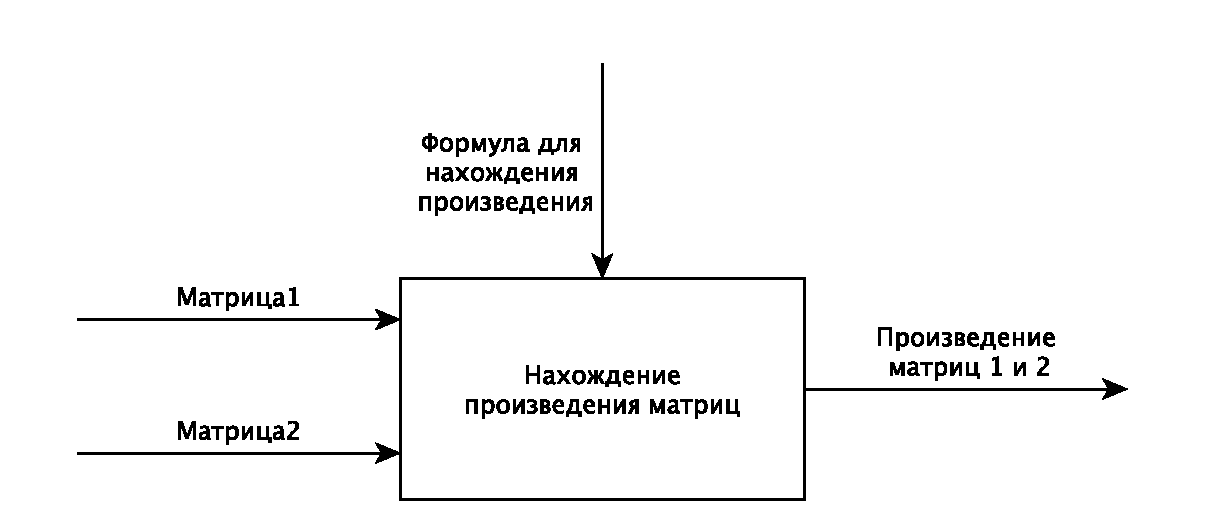
\includegraphics[scale = 0.8]{idef0} \\ Рис.  1 - Функциональная модель алгоритма нахождения произведения матриц. 
	\end{center}
	
        
        \subsection{Схемы алгоритмов}
        \hfill
        
        Приведем схемы 3 исследуемых алгоритмов (см. рисунки 2-4). 
        
        \hfill
        \paragraph{Стандартный алгоритм}
        
        \begin{center}
        		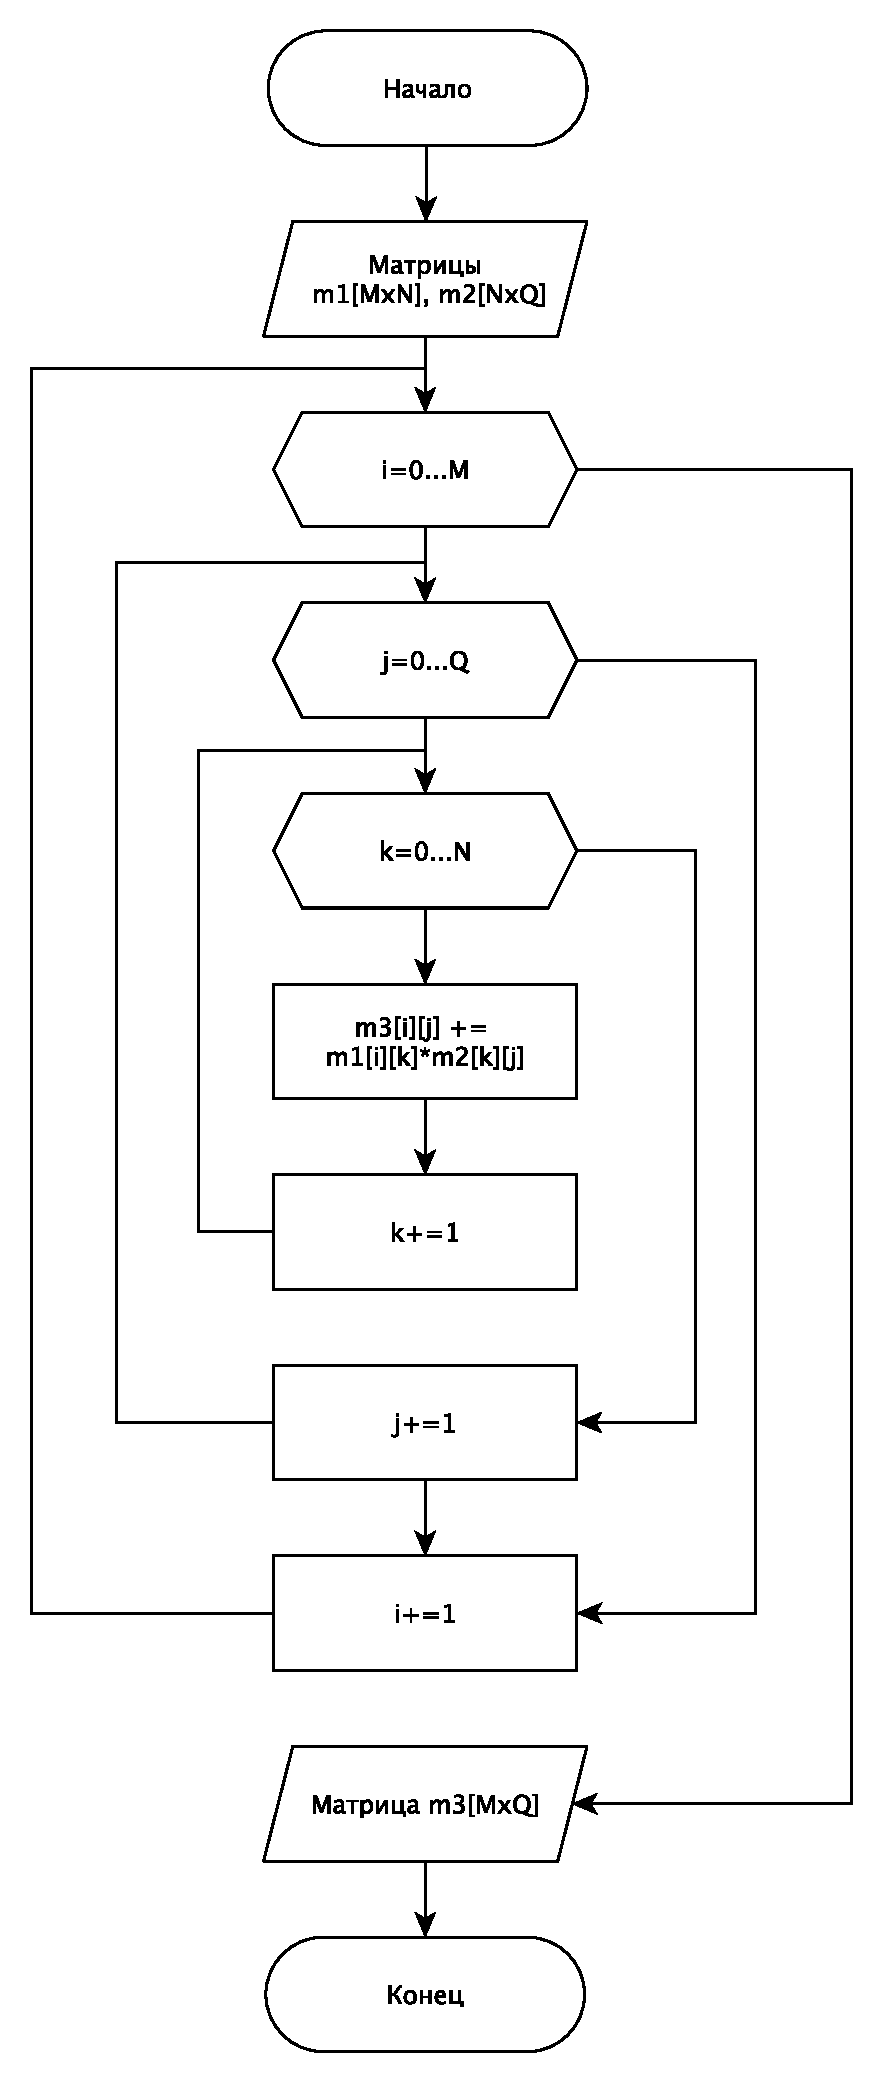
\includegraphics[scale = 0.65]{shema1} \\ Рис. 2 - Алгоритм нахождения произведения матриц стандартным методом
	\end{center}
	
	\hfill
        \paragraph{Алгоритм Винограда}
        
        \begin{center}
        		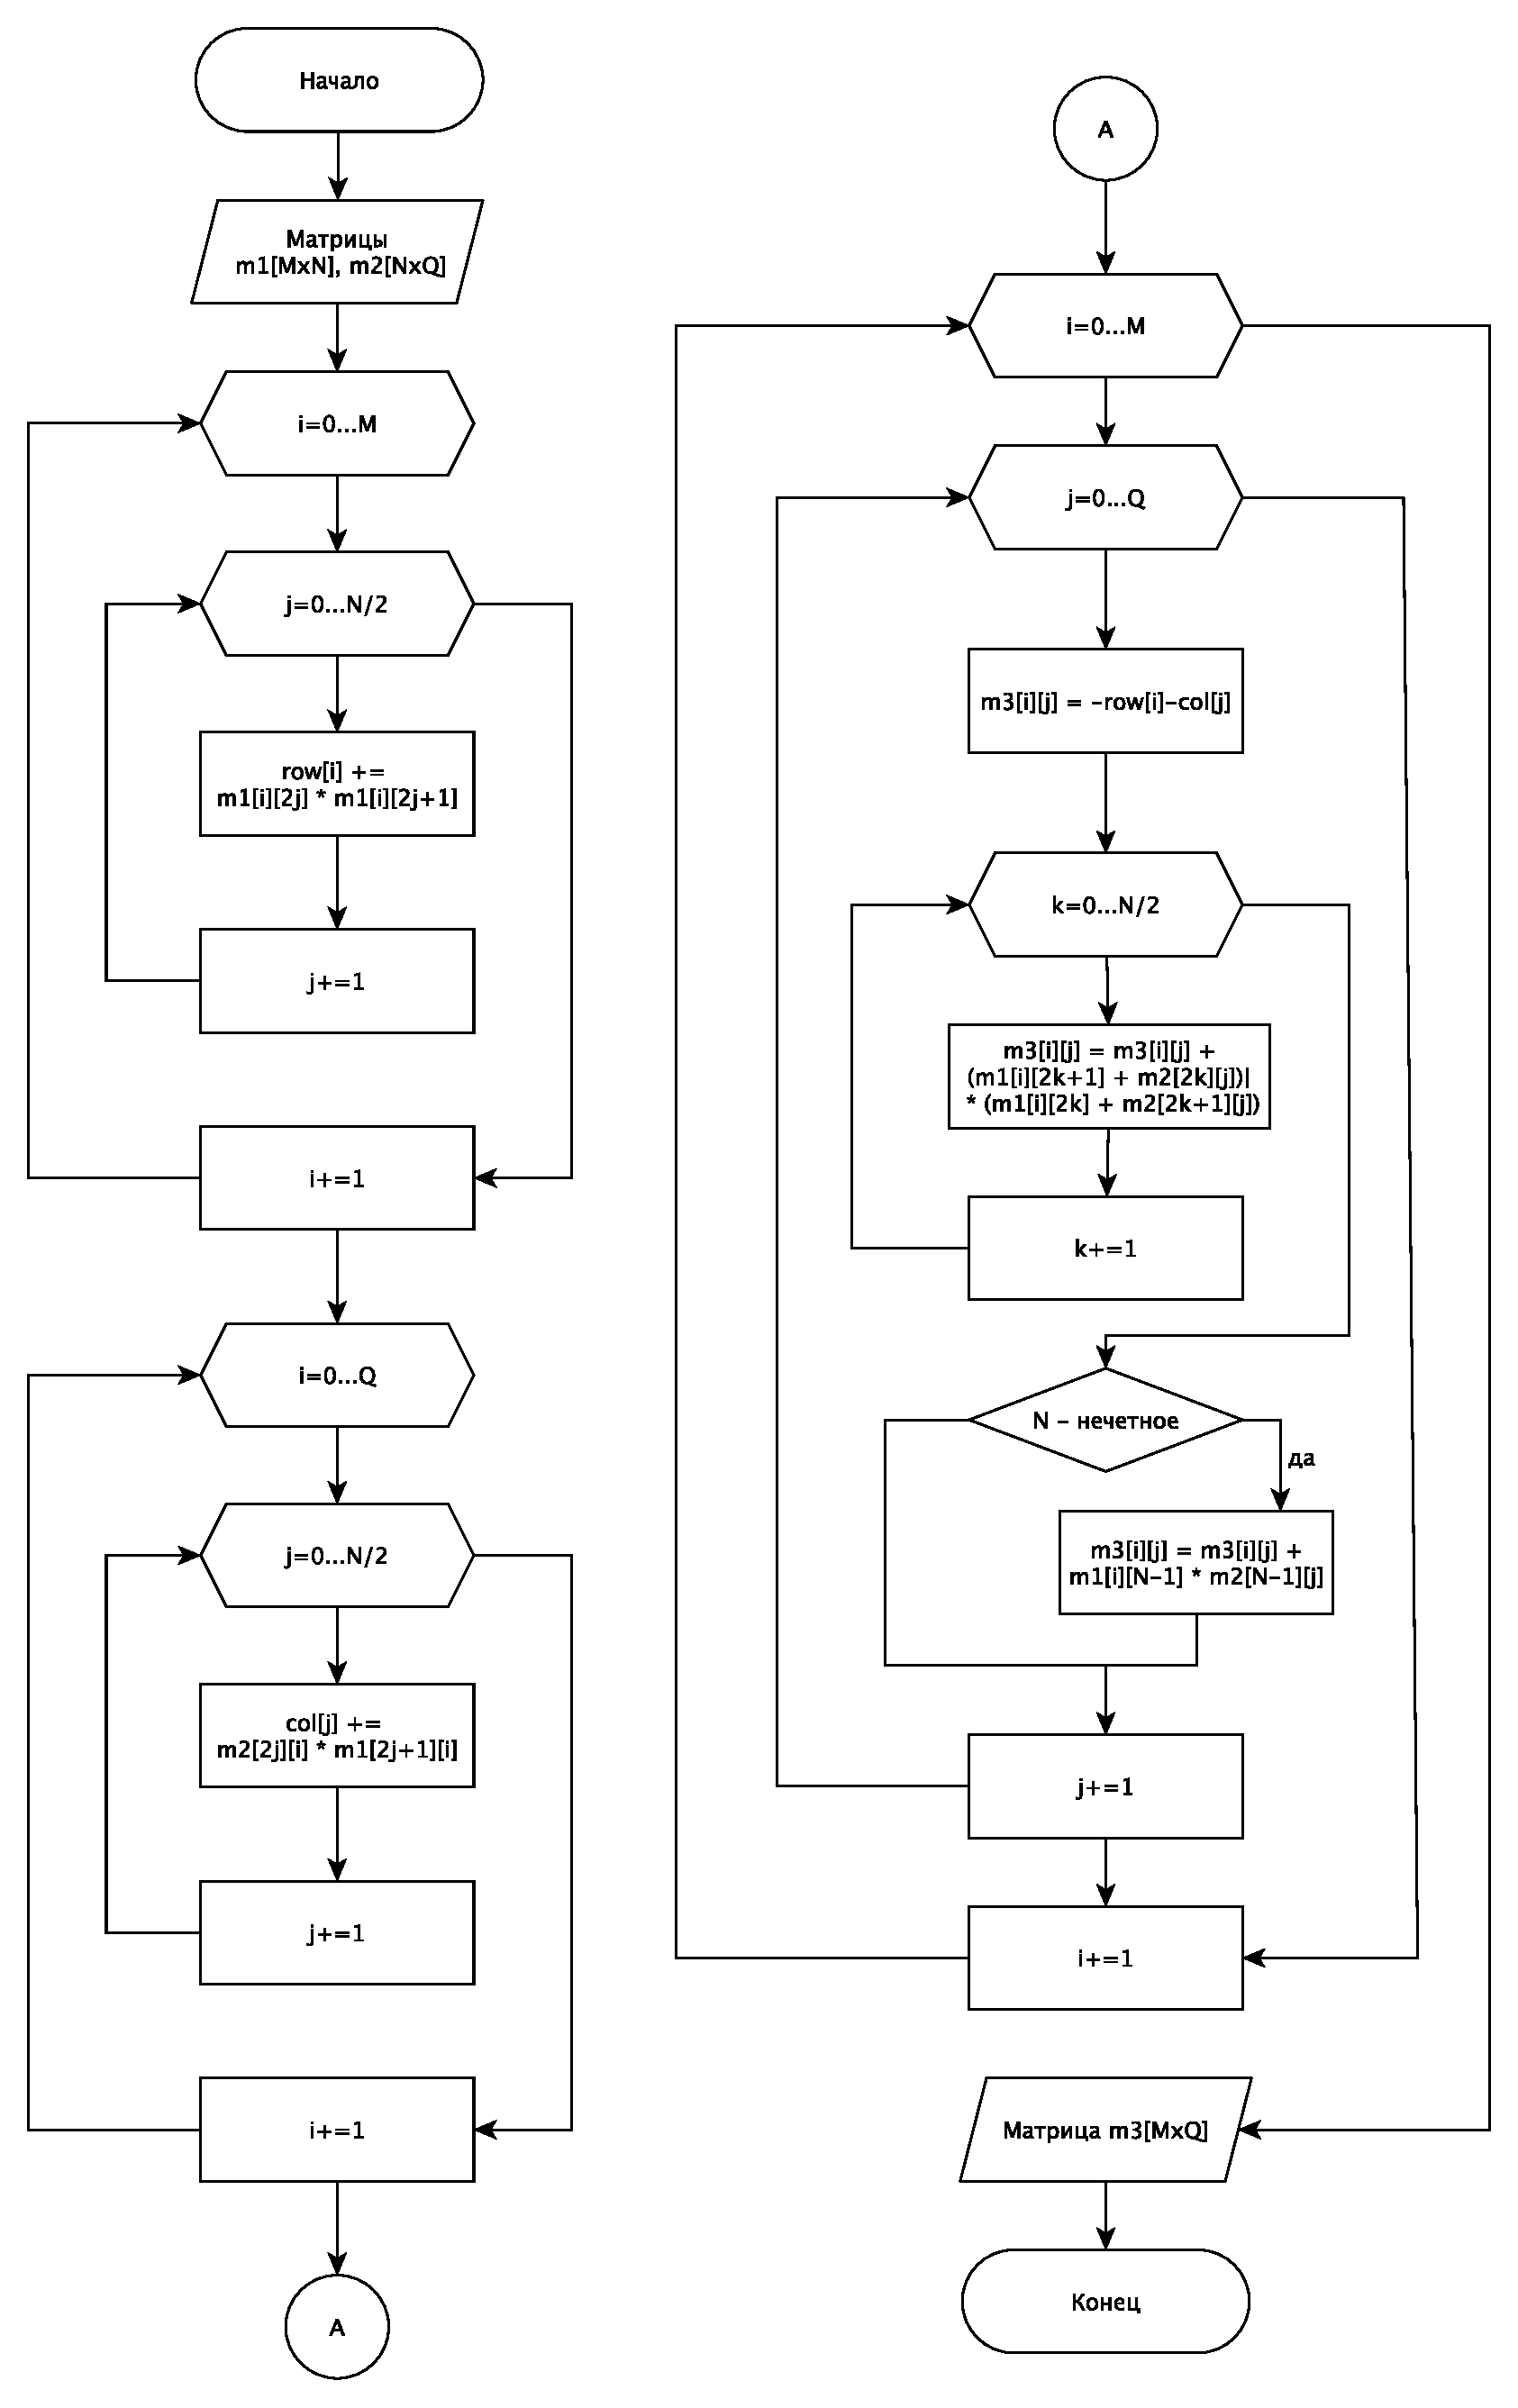
\includegraphics[scale = 0.53]{shema2} \\ Рис. 3 - Алгоритм нахождения произведения матриц методом Винограда
	\end{center}
	
	\hfill
	\paragraph{Алгоритм Винограда с оптимизациями}
	
	\begin{center}
        		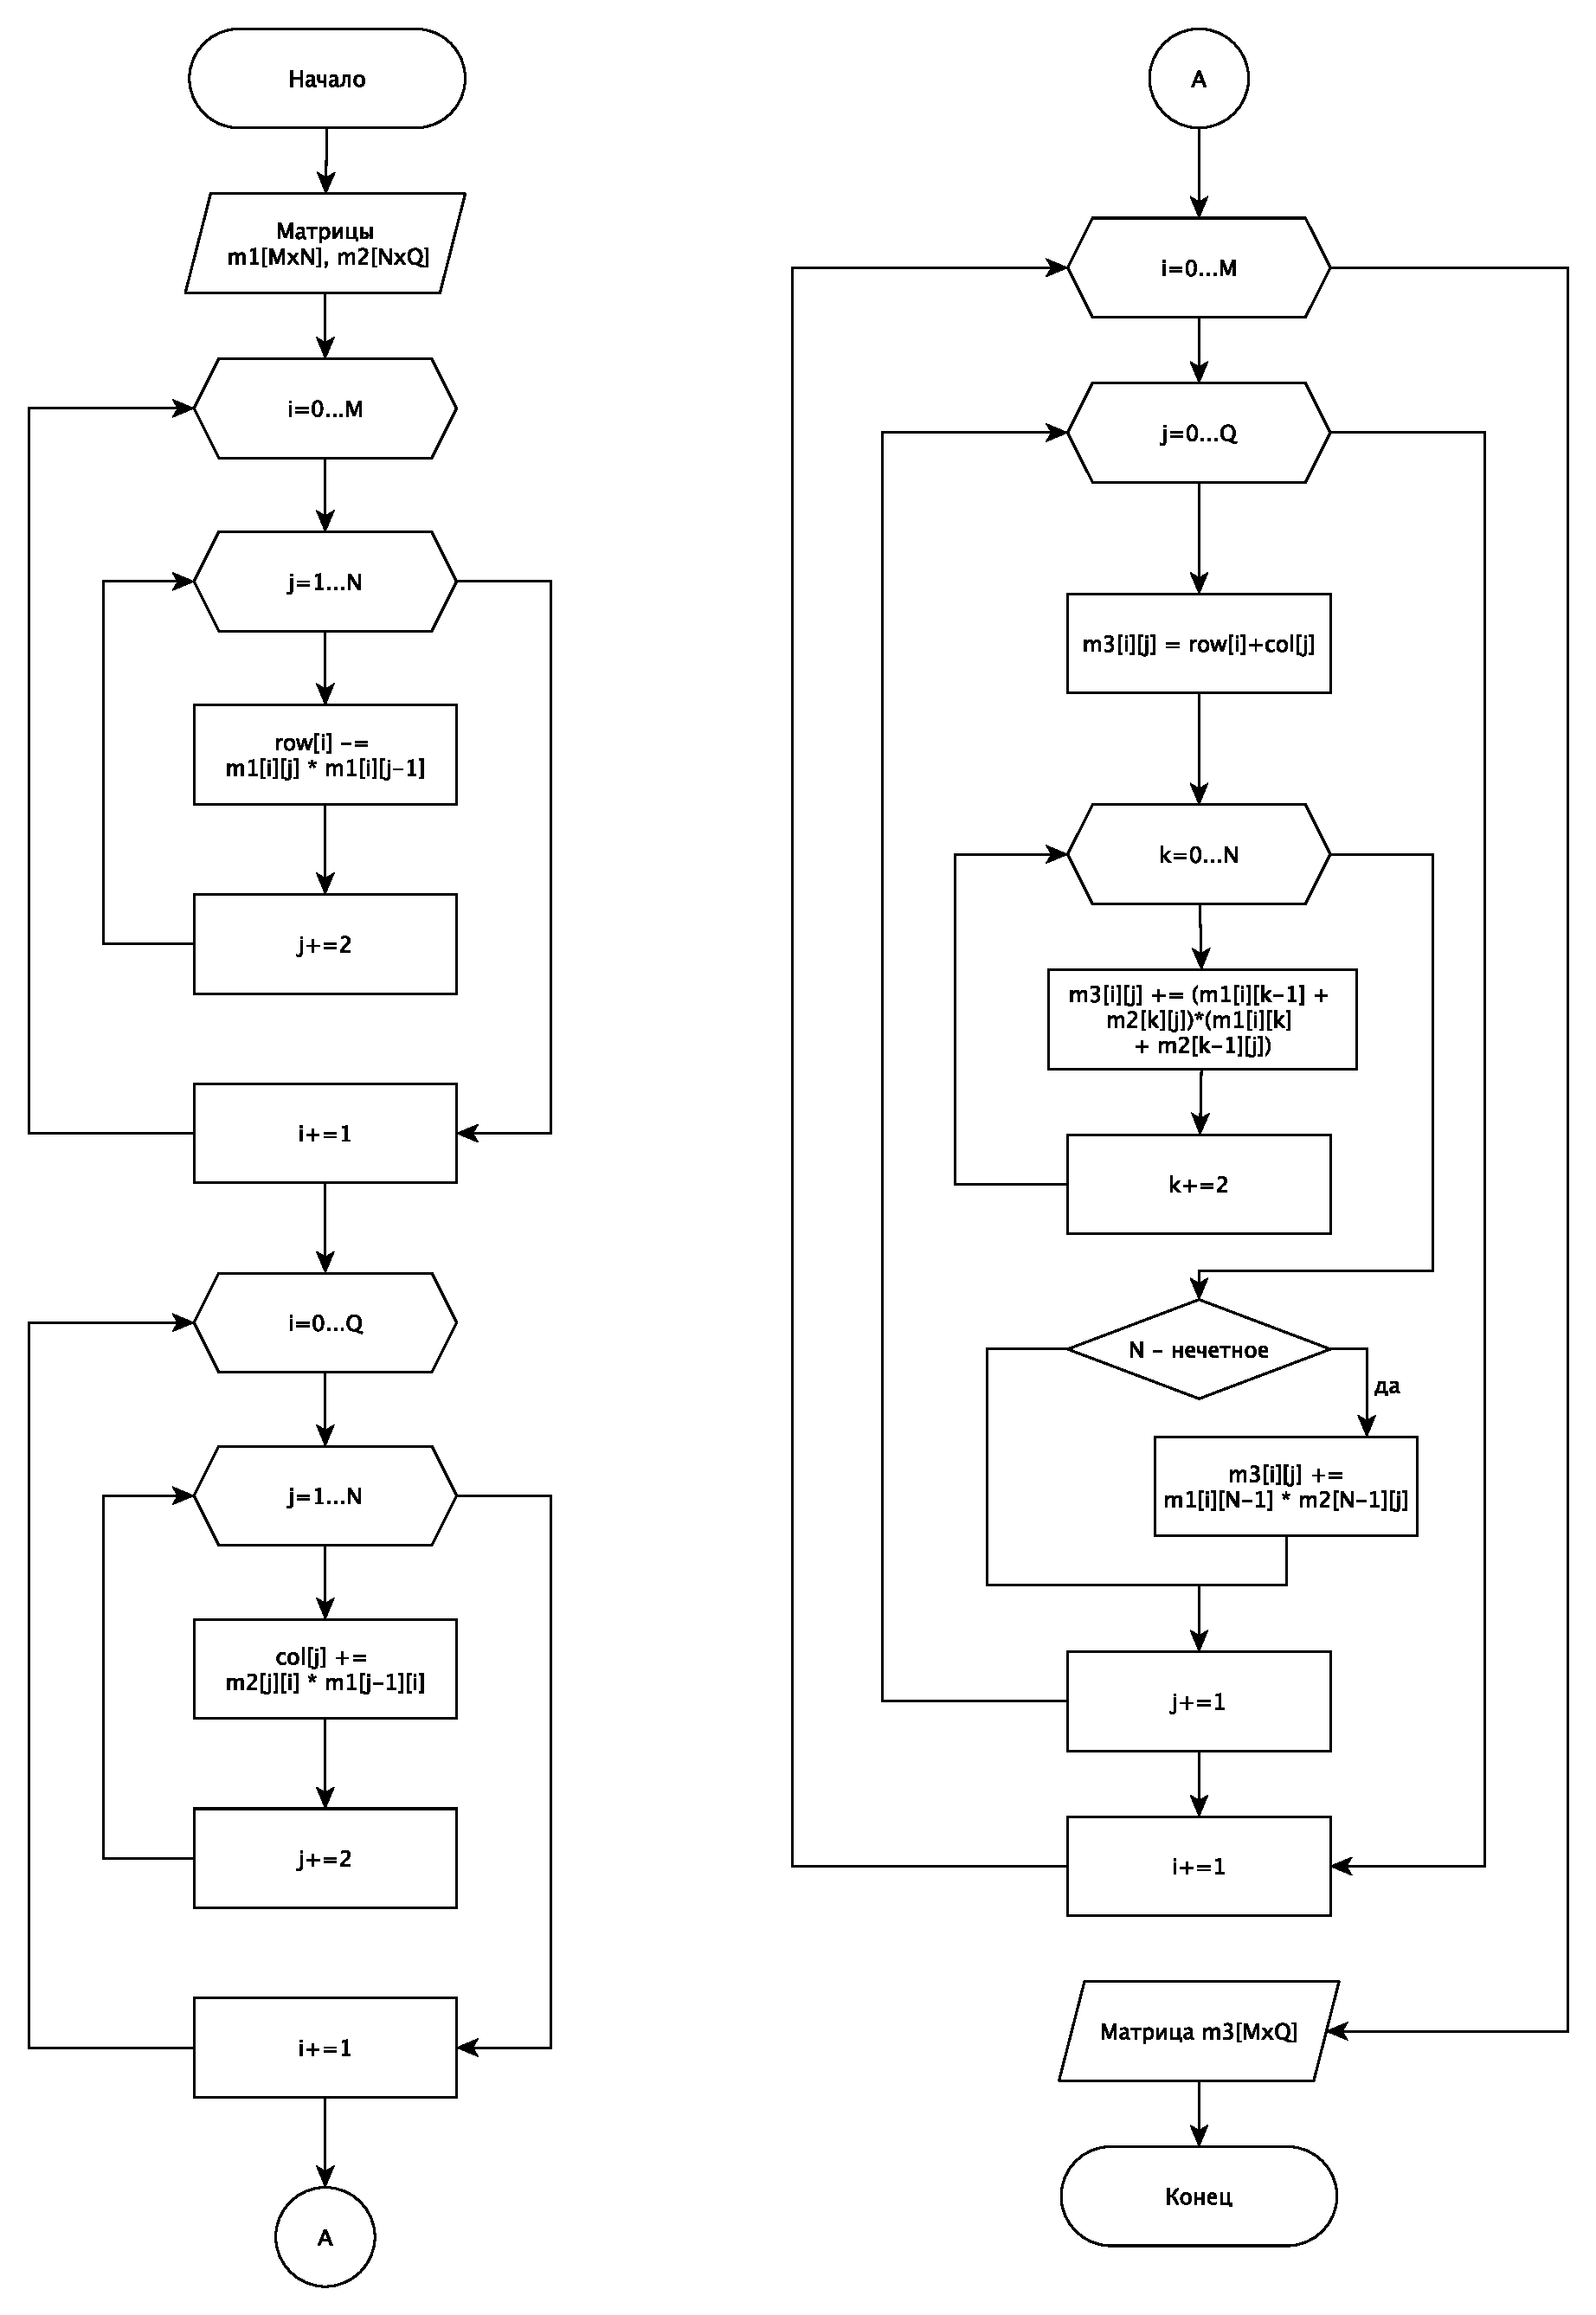
\includegraphics[scale = 0.53]{shema3} \\ Рис. 4 - Алгоритм нахождения произведения матриц методом Винограда с оптимизациями
	\end{center}	
	
	\hfill
	
	\textbf{Произведем теоретическую оценку трудоемкости алгоритмов умножения матриц}
	\begin{enumerate}
		\item Стандартный алгоритм
		$$f=2+M(2+2+Q(2+2+N(2+8+1+1+1)))=13MNQ+4MQ+4M+2$$
		Оценка трудоемкости приближается к наиболее растущим слагаемым, здесь куб линейного размера матриц. 
		\item Алгоритм Винограда
		
		Предназначен для снижения доли умножения
		
		$$c_{ij}=\underbrace{u_1u_2u_3u_4}_{\vec{u}}*
		\underbrace{\begin{pmatrix} 
    			v_1 \\
   			v_2 \\ 
   			v_3 \\ 
    			v_4
  		\end{pmatrix}}_{\vec{v}}=u_1v_1+u_2v_2+u_3v_3+u_4v_4=(u_1+v_2)(u_2+v_1)+(u_3+v_4)(u_4+v_3)-\underbrace{u_1u_2-u_3u_4-v_1v_2-v_3v_4}_{\text{Вычисляется заранее для строк}}
		$$
		Таким образом, трудоемкость:
		$$f=2+M(2+2+Q(2+4+3+3+N/2(3+12+11)))=13MNQ+12MQ+4M+2$$
		
		Доля умножения меньше чем в стандартном. 
		
		\item Алгоритм Винограда с соответствующими оптимизациями
		
		 Введем оптимизации: 
		 \begin{enumerate}
		 	\item+=
			\item j<N, j+=2 
			\item Считаем суммы уже отрицательными
		\end{enumerate}
		
		Тогда трудоемкость:
		$$f=2+M(2+2+Q(2+6+2+N/2(2+3+7+6)))=9MNQ+10MQ+4M+2$$
		
		Доля умножения меньше чем в стандартном. 
	\end{enumerate}

	
	\subsection{Выводы}
	\hfill
	
	Несмотря на сложность алгоритма Винограда по сравнению со стандартным, доля умножения в алгоритме Винограда меньше и по расчетам из аналитической части, трудоемкость меньше. 
	
	Также, необходимо обратить внимание на то, что при работе алгоритма Винограда с матрицами нечетной размерности, необходимо произвести дополнительные действия, в то время как алгоритм стандартный не зависит от четности размерности матриц. 
	
	Необходимо разработать данные алгоритмы и убедиться в корректности наших предположений. 
	
    	\newpage

        \section{Технологическая часть}
        \hfill
        
        Стоит задача разработки и сравнительного анализа алгоритмов, вычисляющих произведения матриц. 
        \hfill
        
        В реализациях в целях увеличения точности подсчета времени вывод матрицы был вынесен за пределы функций-алгоритмов. В целях наглядности были опущены части программ, не относящиеся к работе алгоритмов.
        
        \hfill

        \subsection{Требования к программному обеспечению}
        \hfill
        
        ПО должно предоставлять возможность замеров процессорного времени выполнения реализации каждого алгоритма. Требуется провести замеры для варьирующихся размеров матриц: от 100 до 1000 и от 101 до 1001. Один эксперимент ставится не менее 100 раз, результат одного эксперимента рассчитывается как среднее значение результатов проведенных испытаний с одинаковыми входными данными.
        \hfill
        
        \subsection{Средства реализации}
        \hfill
        
        В качестве языка программирования был выбран Python[8], так как я знакома с этих языком программирования. 
        \hfill
        
        Для замеров времени была выбран метод $process\_time()$, возвращает текущее время процессора как число с плавающей запятой, выраженное в секундах в Unix.
        \hfill
        
        Для генерации случайных матриц, заданного размера использовался метод $randint()$. 
        \hfill
        
        \subsection{Листинг кода}
        \hfill
        
        	\textbf{Стандартный алгоритм:}
        
	\begin{lstlisting}
	for i in range(0, m):
            for j in range(0, q):
                for k in range(0, n):
                    m3[i][j] = m3[i][j] + m1[i][k] * m2[k][j]
	\end{lstlisting}

	\textbf{Алгоримт Винограда: }
	\begin{lstlisting}
	row = [0] * m
        for i in range(0, m):
            for j in range(0, n // 2, 1):
                row[i] = row[i] + m1[i][2 * j] * m1[i][2 * j + 1]

        col = [0] * q
        for j in range(0, q):
            for i in range(0, n // 2, 1):
                col[j] = col[j] + m2[2 * i][j] * m2[2 * i + 1][j]

        start_time = time.process_time()
        for i in range(0, m):
            for j in range(0, q):
                m3[i][j] = -row[i] - col[j]
                for k in range(0, n // 2, 1):
                    m3[i][j] = m3[i][j] + (m1[i][2 * k + 1] + m2[2 * k][j]) 
                    * (m1[i][2 * k] + m2[2 * k + 1][j])
                if 1 == n % 2:
                    m3[i][j] = m3[i][j] + m1[i][n - 1] * m2[n - 1][j]
	\end{lstlisting}

	\textbf{Алгоритм Винограда с оптимизациями: }
	\begin{lstlisting}
	row = [0] * m
        for i in range(0, m):
            for j in range(1, n, 2):
                row[i] -= m1[i][j] * m1[i][j - 1]

        col = [0] * q
        for j in range(0, q):
            for i in range(1, n, 2):
                col[j] -= m2[i][j] * m2[i - 1][j]

        start_time = time.process_time()
        for i in range(0, m):
            for j in range(0, q):
                m3[i][j] = row[i] + col[j]
                for k in range(1, n, 2):
                    m3[i][j] += (m1[i][k - 1] + m2[k][j]) * (m1[i][k] + m2[k - 1][j])
                if 1 == n % 2:
                    m3[i][j] += m1[i][n - 1] * m2[n - 1][j]
	\end{lstlisting}
        
	\subsection{Тестирование}
	\hfill
	
	В таблице 1 представлена заготовка данных для тестирования наших алгоритмов. 
	\begin{center}
		\begin{tabular}{  | c | c | c | }
			\hline
			\textbf{Матрица1} & \textbf{Матрица2} & \textbf{Ожидаемый результат} \\ \hline
			$\begin{bmatrix} 
   			1&2&3 \\
    			4&5&6 \\ 
   			7&8&9 \\ 
			\end{bmatrix}$ & 
			$\begin{bmatrix} 
   			1&2&3 \\
    			4&5&6 \\ 
   			7&8&9 \\ 
			\end{bmatrix}$ &
			$\begin{bmatrix} 
   			30&36&42 \\
    			66&81&96 \\ 
   			102&126&150 \\ 
			\end{bmatrix} $ \\ \hline
			
			$\begin{bmatrix} 
   			1&2&3 \\
    			4&5&6 \\ 
   			7&8&9 \\ 
			\end{bmatrix}$ & 
			$\begin{bmatrix} 
   			1&2&3 \\
    			4&5&6 \\ 
			\end{bmatrix}$ &
			$\text{Матрицы не могут быть перемножены}$ \\ \hline
			
			$\begin{bmatrix} 
   			1&2 \\
    			4&5 \\ 
   			7&8 \\ 
			\end{bmatrix}$ & 
			$\begin{bmatrix} 
   			1&2&3 \\
    			4&5&6 \\ 
			\end{bmatrix}$ &
			$\begin{bmatrix} 
   			9&12&15 \\
    			24&33&42 \\ 
   			39&54&69 \\ 
			\end{bmatrix} $ \\ \hline
		\end{tabular}
		
		\hfill
		
		Таблица 1.
		Подготовленные тестовые данные.  
	\end{center}
	
	\subsection{Выводы}
	\hfill
	
	Реализовано 3 алгоритма, подготовлены тесты для оценки качества их работы. 
        
        Получены практические навыки реализации алгоритмов матричного умножения: стандартного и Винограда. 
	
        \hfill
        
        
        \newpage

        \section{Экспериментальная часть}
       
        
        \subsection{Примеры работы}
	\hfill
	
	На рисунке 5 представлены примеры работы программы на разных входных данных. 
	\begin{figure}[ht]\center
		\begin{tabular}{cc}
			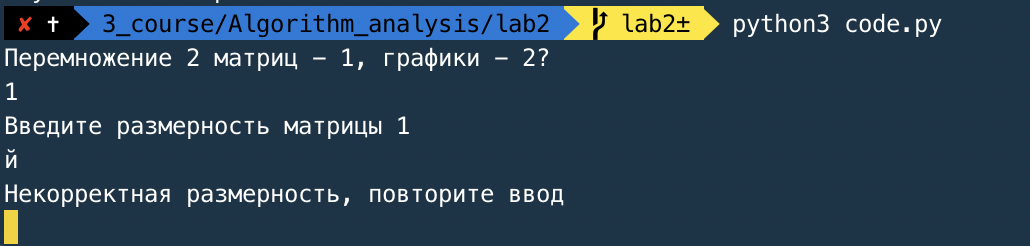
\includegraphics[width=80mm]{ex1} & 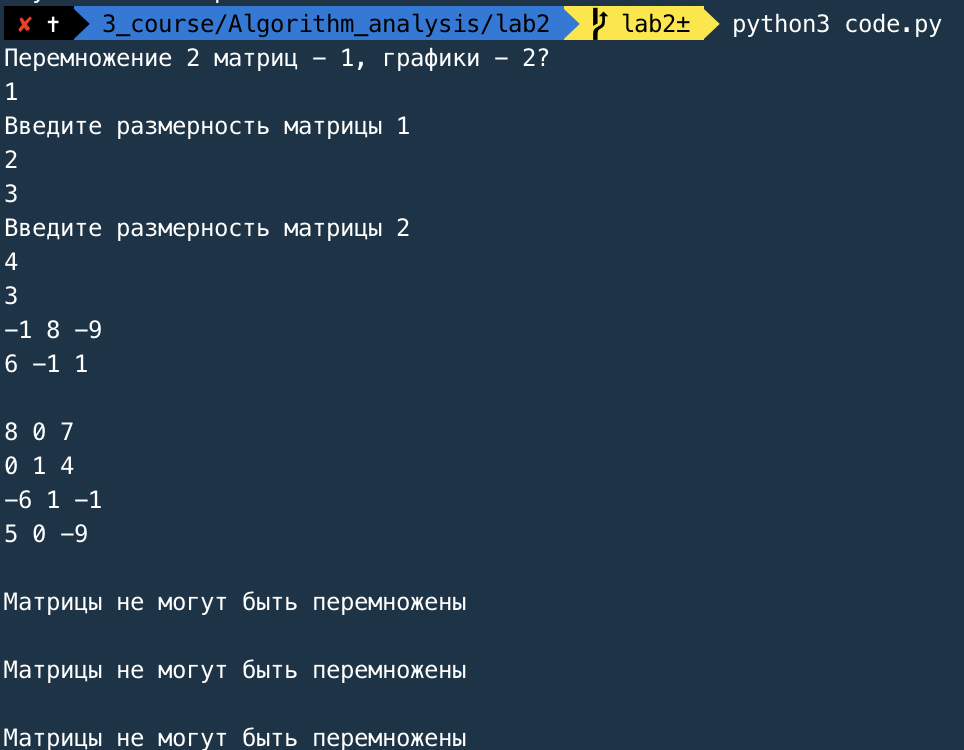
\includegraphics[width=80mm]{ex2} \\
			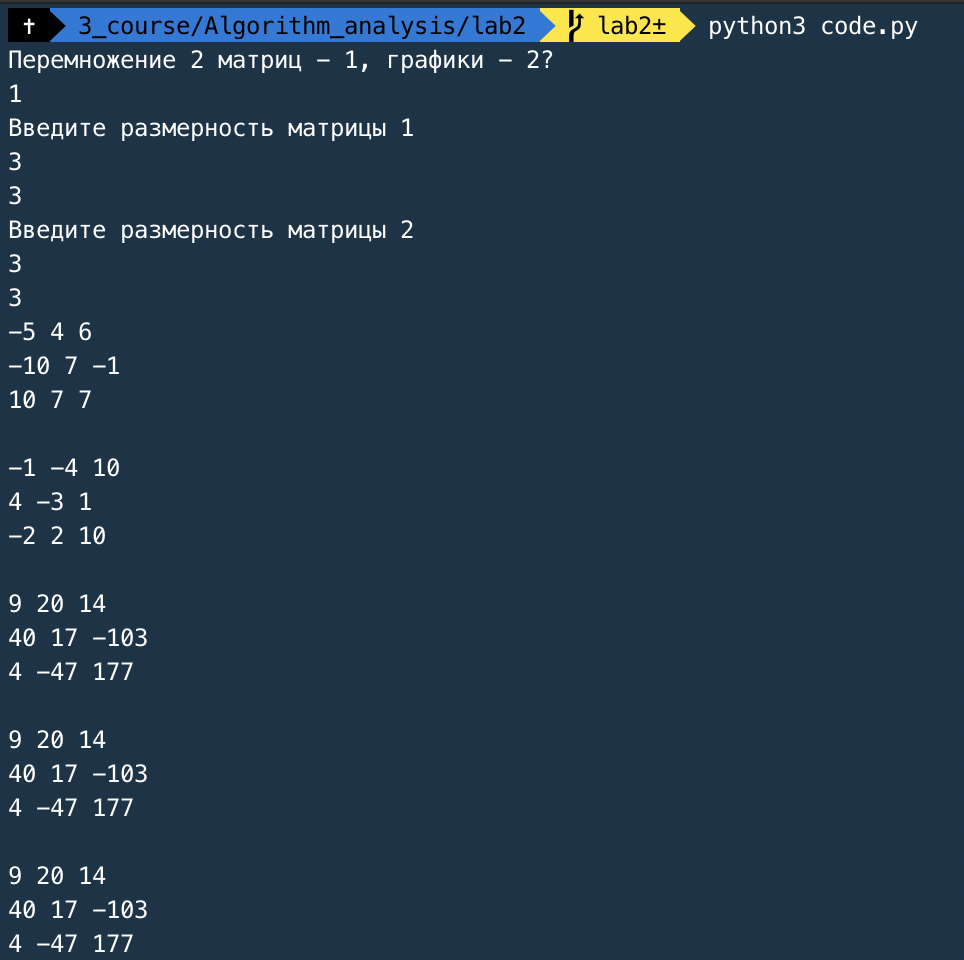
\includegraphics[width=80mm]{ex3} & 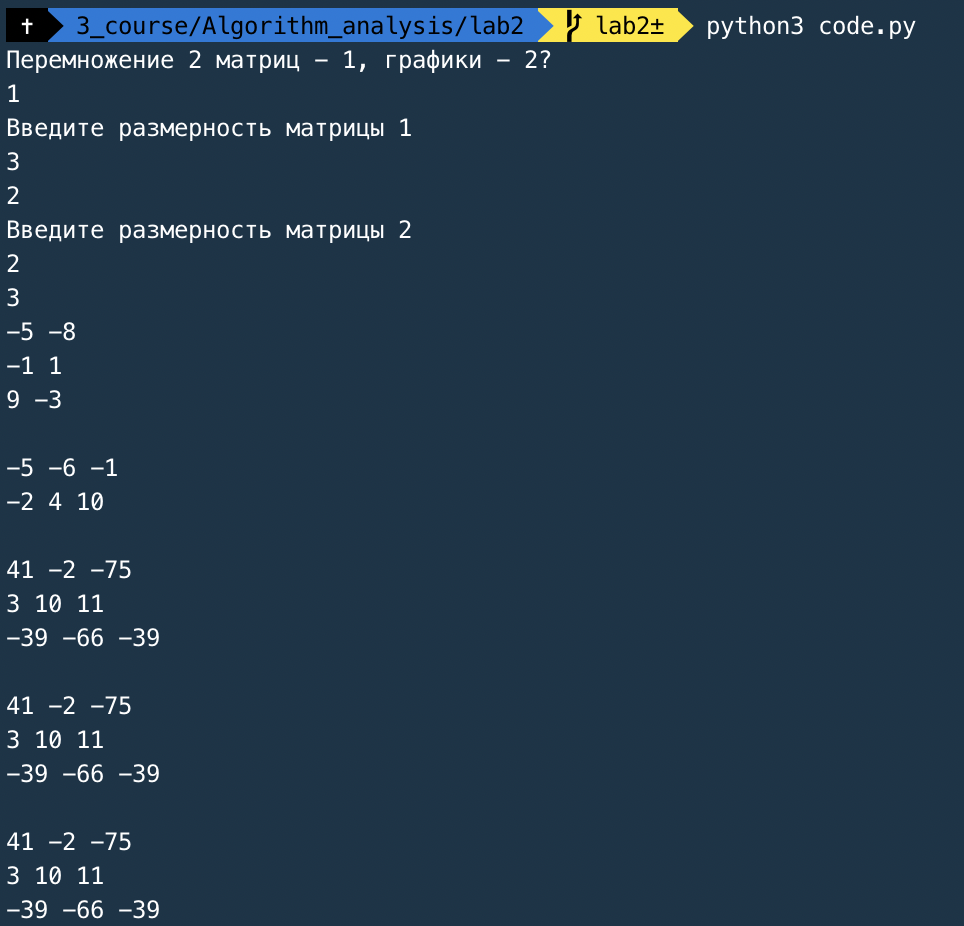
\includegraphics[width=80mm]{ex4}
		\end{tabular}
		\\ Рис. 5 - Примеры работы
	\end{figure}
	        
        \subsection{Результаты тестирования}
        
	\hfill
	Проверяем нашу программу на тестах из таблицы 1. Полученные результаты представлены в таблице 2. 
	\begin{center}
		\begin{tabular}{ | c | c | c | c | c |}
			\hline
			\textbf{Матрица1} & \textbf{Матрица2} & \textbf{Стандартный} & \textbf{Виноград} & \textbf{Виноград с оптимизациями} \\ \hline
			$\begin{bmatrix} 
   			1&2&3 \\
    			4&5&6 \\ 
   			7&8&9 \\ 
			\end{bmatrix}$ & 
			$\begin{bmatrix} 
   			1&2&3 \\
    			4&5&6 \\ 
   			7&8&9 \\ 
			\end{bmatrix}$ &
			$\begin{bmatrix} 
   			30&36&42 \\
    			66&81&96 \\ 
   			102&126&150 \\ 
			\end{bmatrix} $ &
			$\begin{bmatrix} 
   			30&36&42 \\
    			66&81&96 \\ 
   			102&126&150 \\ 
			\end{bmatrix} $ &
			$\begin{bmatrix} 
   			30&36&42 \\
    			66&81&96 \\ 
   			102&126&150 \\ 
			\end{bmatrix} $ \\ \hline
			
			$\begin{bmatrix} 
   			1&2&3 \\
    			4&5&6 \\ 
   			7&8&9 \\ 
			\end{bmatrix}$ & 
			$\begin{bmatrix} 
   			1&2&3 \\
    			4&5&6 \\ 
			\end{bmatrix}$ &
			$\begin{matrix} 
   			\text{Матрицы не могут} \\
    			\text{быть перемножены} \\ 
			\end{matrix} $ &
			$\begin{matrix} 
   			\text{Матрицы не могут} \\
    			\text{быть перемножены} \\ 
			\end{matrix} $ &
			$\begin{matrix} 
   			\text{Матрицы не могут} \\
    			\text{быть перемножены}\\ 
			\end{matrix} $ \\ \hline
			
			$\begin{bmatrix} 
   			1&2 \\
    			4&5 \\ 
   			7&8 \\ 
			\end{bmatrix}$ & 
			$\begin{bmatrix} 
   			1&2&3 \\
    			4&5&6 \\ 
			\end{bmatrix}$ &
			$\begin{bmatrix} 
   			9&12&15 \\
    			24&33&42 \\ 
   			39&54&69 \\ 
			\end{bmatrix} $ &
			$\begin{bmatrix} 
   			9&12&15 \\
    			24&33&42 \\ 
   			39&54&69 \\ 
			\end{bmatrix} $ &
			$\begin{bmatrix} 
   			9&12&15 \\
    			24&33&42 \\ 
   			39&54&69 \\ 
			\end{bmatrix} $ \\ \hline
		\end{tabular}
		
		\hfill
		
		Таблица 2.
		Тестирование программы.  
	\end{center}
	
	
	\textbf{Тесты пройдены}

	\subsection{Замеры времени}
	\hfill
	
	На графиках 6-7 представлено сравнение алгоритмов умножения матриц. 
	\begin{center}
        		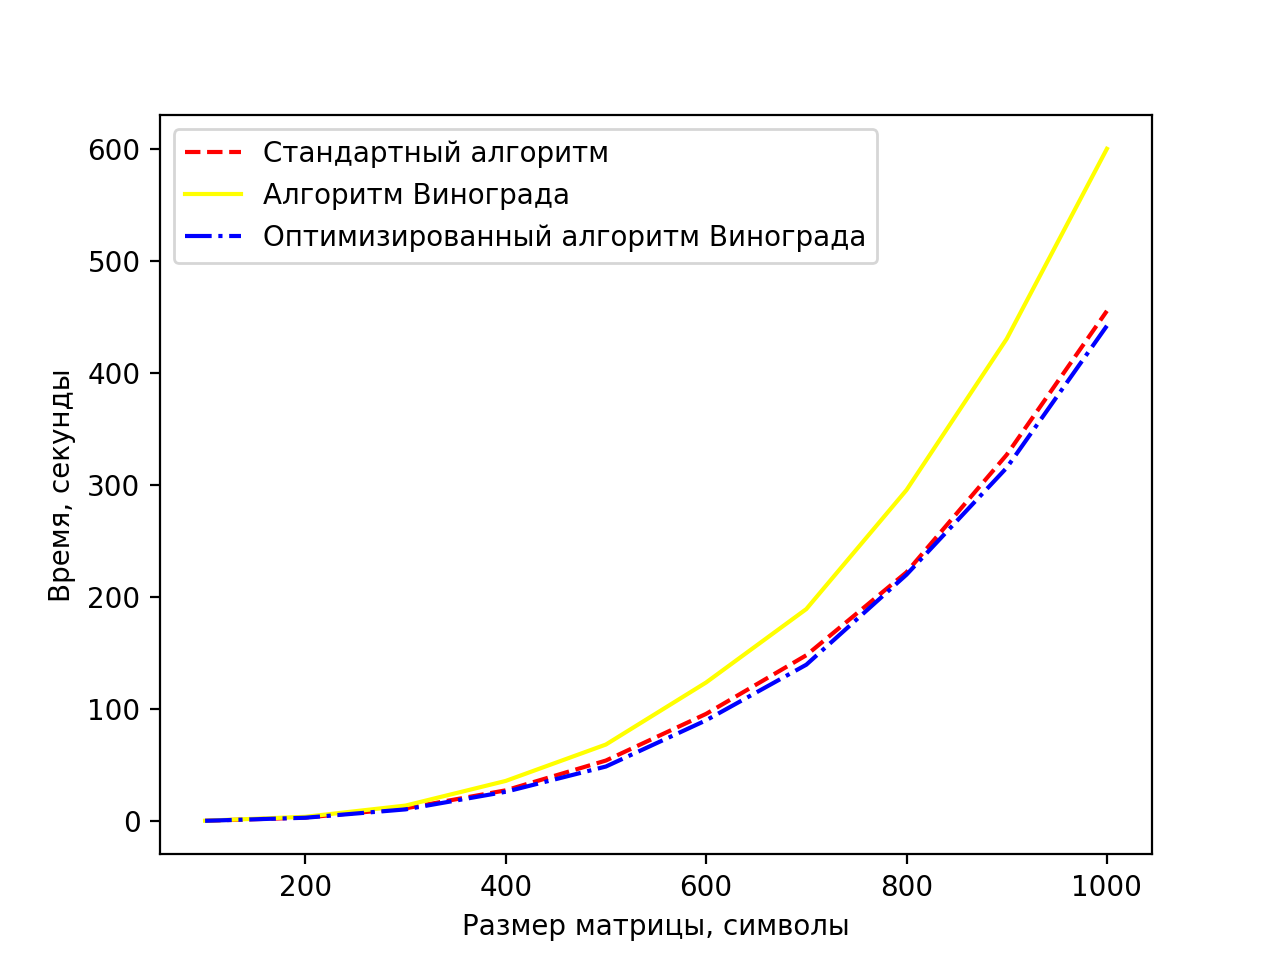
\includegraphics[scale = 1]{graph1} \\ Рис. 6 - Сравнение реализации алгоритмов нахождения произведения матриц при четных размерностях
	\end{center}
	
	\begin{center}
        		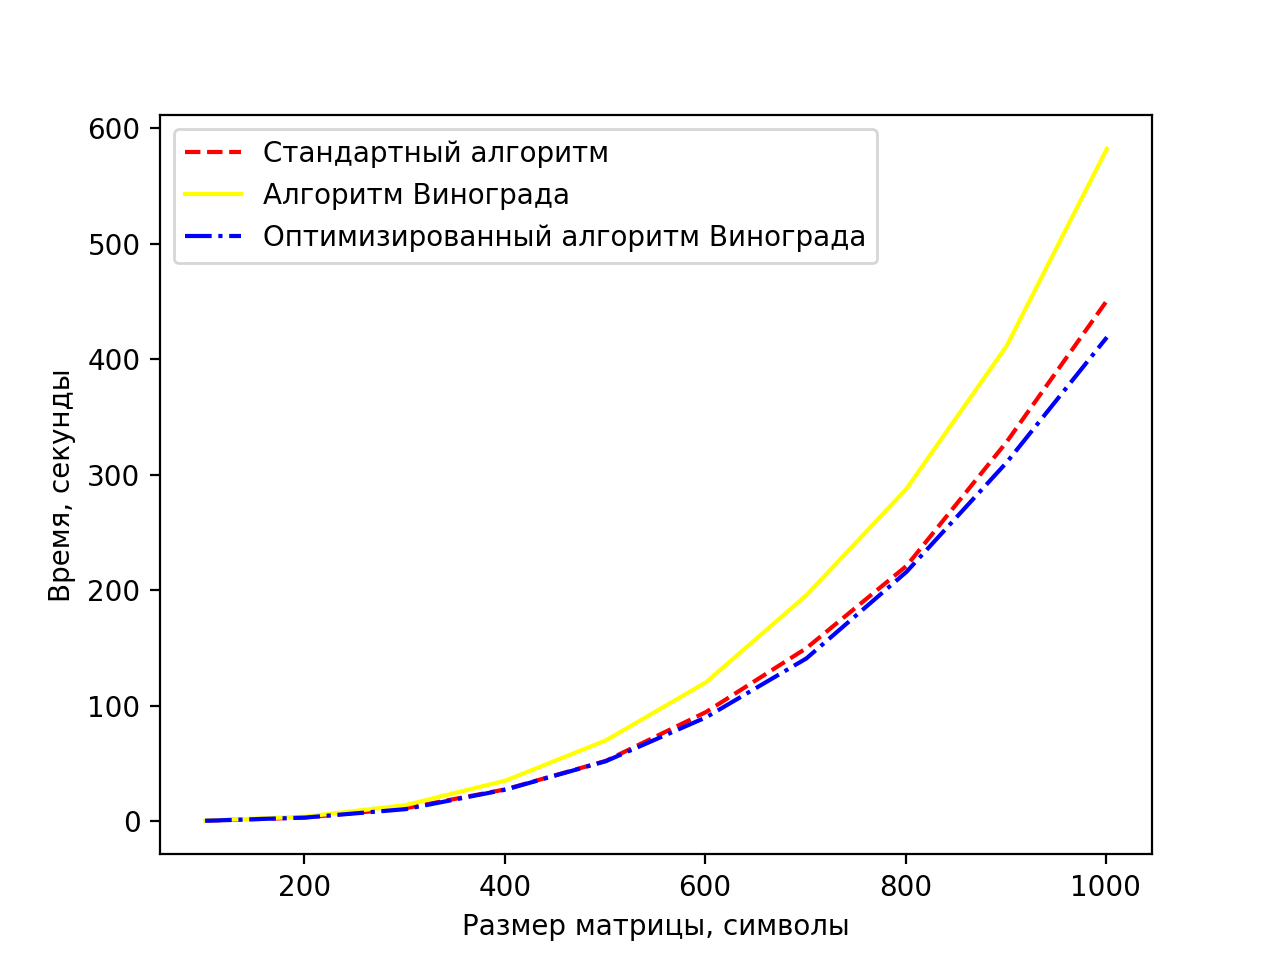
\includegraphics[scale = 1]{graph2} \\ Рис. 7 - Сравнение реализации алгоритмов нахождения произведения матриц при нечетных размерностях
	\end{center}
	
	\subsection{Выводы}
	\hfill
	
	Как мы видим из графиков предположения о более быстрой работе Стандартного алгоритма по сравнению с Виноградом подтвердились, время вычислений меньше на 25\%. Но в плюсах использования алгоритма Винограда, это сокращение операции умножения. 
	
	Однако алгоритм Винограда с оптимизациями работает примерно также, как и стандартный, с этим связана оценка трудоемкости операции +=, оказывается в языке программирования Python эта операция выполняется гораздо дольше обычного сложения и присваивания.
	
	Также при сравнении работы для лучших случаев у Винограда (лучшие при четном размере матрицы) и худших (при нечетном) разница не значительна. 
	
	Пример сравнения скорости работы для цикла с 10000000 итераций представлен на рисунке 8. Из него видно, что трудоемкость операции += выше на 50 \%. 
	
	\begin{center}
		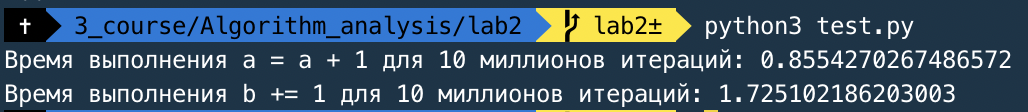
\includegraphics[scale = 0.8]{test} \\ Рис. 8 - Сравнение работы операции += и обычного присваивания со сложением
	\end{center}

   	\newpage

        \anonsection{Заключение}
        
        \hfill
        
        В данной лабораторной работе было реализовано и пронализировано 3 алгоритма нахождения произведения 2 матриц:
	\begin{enumerate}
	 	\item стандартный алгоритм 
		\item алгоритм Винограда
		\item алгоритм Винограда с модификациями 
	\end{enumerate}
	
	\hfill
	
	Матрицы и матричное умножение активно применяется:
	\begin{enumerate}
		\item в сверточных слоях нейронных сетей для реализации прямого и обратного распространения сигнала
		\item в физике и математике для записи данных и их преобразования
		\item в компьютерной графике, для отображения изображений и их преобразований
		\item в психологии, для анализа результатов тестов
		\item в экономике, биологии, химии и других науках. 
	\end{enumerate}
	
	\hfill
	
	При сравнении данных алгоритмов пришли к следующим выводам:
	\begin{enumerate}
 		\item Самым быстрым  является алгоритм винограда, опережающий стандартный на 25\%. 
 		\item Оптимизированный алгоритм Винограда проигрывает из-за трудоемкости операции += в Python. 
	\end{enumerate}
	
	\hfill
	
	В данной лабораторной работе выполнены следующие задачи. 
        \begin{enumerate} 
		\item Изучены алгоритмов умножения матриц: стандартный, Винограда и Винограда с оптимизациями. 
		\item Произведена оценка трудоемкости алгоритмов умножения матриц, лучших и худших случаев с условием их наступления. 
		\item Получены практические навыки реализации данных алгоритмов на одном из языков программирования. 
		\item Проведен сравнительный анализ алгоритмов по затрачиваемым ресурсам (зависимость времени от длины строки). 
		\item Экспериментально подтверждено различие в трудоемкости алгоритмов с указанием лучшего и худшего случаев. 
	\end{enumerate}
        

 	\newpage

        \begin{thebibliography}{}
        		\bibitem{} [Электронный ресурс]. - Режим доступа: http://poivs.tsput.ru/ru/Math/Algebra/LinearAlgebra/Matrices (дата обращения: 08.10.2019)
		\bibitem{}  [Электронный ресурс]. - Режим доступа: https://habr.com/ru/post/359272/(дата обращения: 08.10.2019)
		\bibitem{}  [Электронный ресурс]. - Режим доступа: https://urok.1sept.ru/статьи/637896/(дата обращения: 08.10.2019)
		\bibitem{}  [Электронный ресурс]. - Режим доступа: http://we.easyelectronics.ru/Theory/cifrovye-rekursivnye-filtry-chast-1.html(дата обращения: 08.10.2019)
		\bibitem{}  [Электронный ресурс]. - Режим доступа: http://window.edu.ru/resource/898/72898/files/stup559.pdf(дата обращения: 08.10.2019)
		\bibitem{}  [Электронный ресурс]. - Режим доступа: http://vekkv.ru/holotropnoe-dyhanie-transpersonalnaya-psihologiya/1859/(дата обращения: 08.10.2019)
		\bibitem{} [Электронный ресурс]. - Режим доступа:  https://www.eduherald.ru/ru/article/view?id=14118(дата обращения: 08.10.2019)
		\bibitem{}  [Электронный ресурс]. - Режим доступа: https://cyberleninka.ru/article/n/matrichnyy-printsip-v-biologii-progiloe-nastoyaschee-buduschee(дата обращения: 08.10.2019)
		\bibitem{}  [Электронный ресурс]. - Режим доступа: http://www.chemicals-el.ru/chemicals-2400-1.html(дата обращения: 08.10.2019)
		\bibitem{} Strassen V. Gaussian Elimination is not Optimal // Numer. Math — Springer Science+Business Media, 1969. — Vol. 13, Iss. 4. — P. 354–356. — ISSN 0029-599X; 0945-3245 — doi:10.1007/BF02165411
		\bibitem{} Don Coppersmith and Shmuel Winograd. Matrix multiplication via arithmetic progressions. Journal of Symbolic Computation, 9:251-280, 1990.
	\end{thebibliography} 

\end{document}
